%%%%%%%%%%%%%%%%%%%%%%%%%%%%%%%%%%%%%%%%%%%%%%%%%%%%%%%%%%%%%%%%%%%%%%%%%%%%%%%%%%%%%%%%%%%%%%%%%%
%%  Text of the Lithuanian summary should be written here

% !TEX encoding = UTF-8 Unicode
\pagestyle{plain}
\clearpage %To start in new page

%%%%%%%%%%%%%%%%%%%%%%%%%%%%%%%%%%%%%%%%%%%%%%%%%%%%%%%%%%%%%%%%%%%%%%%%%%%%%%%%%%%%%%%%%%%%%%%%%%
%%  Disertacijos lietuviškas tekstas turi būti rašomas čia.

% Toliau pateikta pavyzdys teksto iš Roko Astrausko disertacijos
\section{SECM modeliavimas oksidacijos-redukcijos konkurencijos režime}
\label{sec:santr_reakc}



\subsection{Matematinis modelis}

Dėl simetrijos aplink centrinę elektrodo ašį modelis užrašomas cilindrinėse koordinatėse. Cilindro formos srityje atliekami SECM matavimai yra pakeisti į 2D sritį \ref{fig:santr_Domain} pav.


\begin{figure}[ht!]
\centering
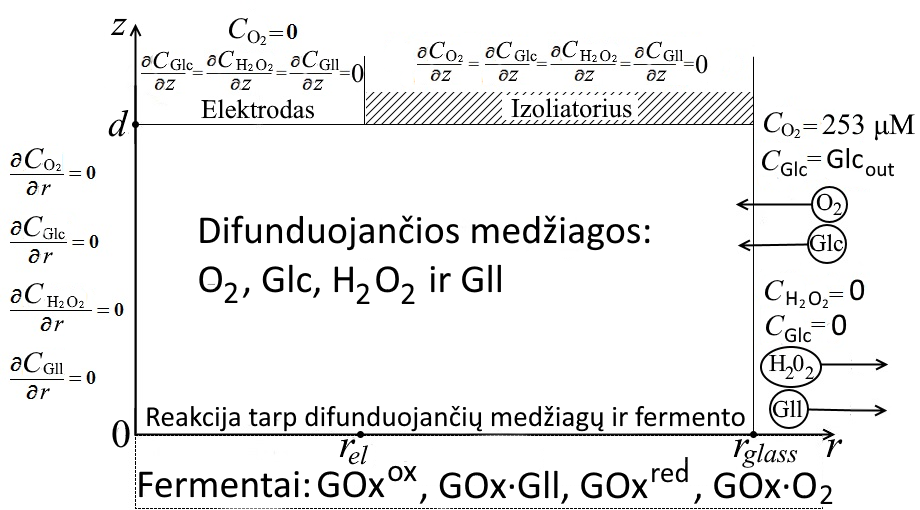
\includegraphics[width=0.8\linewidth]{summary/Model_domainLT.png}
\caption{Modeliavimo srities schema. Pavaizduotos $8$ modeliuotos medžiagos - $4$ difunduojantys reagentai bei $4$ fermento GOx formos, kraštinės sąlygos 4-ioms difunduojančioms medžiagoms ir išorinis srautas.}
\label{fig:santr_Domain}
\end{figure}

Difuzijos procesai išreiškiami antruoju Fiko dėsniu:
\begin{equation}
  \begin{aligned}\label{eq:santr_eq1}
  \frac{\partial C_{O_2}}{\partial t} &= D_{O_2}\,\Delta C_{O_2},\\
  \frac{\partial C_{Glc}}{\partial t} &= D_{Glc}\,\Delta C_{Glc},\\
  \frac{\partial C_{H_2 O_2}}{\partial t} &= D_{H_2 O_2} \,\Delta C_{H_2 O_2},\\
  \frac{\partial C_{Gll}}{\partial t} &= D_{Gll}\,\Delta C_{Gll},  \quad 0<t\leq T,\; 0<z<d,\; 0<r<r_{glass}.
  \end{aligned}
\end{equation}
Šiose lygtyse:
\begin{itemize}
  \item[] $C_{O_2}$, $C_{Glc}$, $C_{H_2 O_2}$ ir $C_{Gll}$ yra atitinkamų difunduojančių re\-a\-gen\-tų koncentracijos, kurios išreiškiamos kaip laiko $t$, er\-dvi\-nių ko\-or\-di\-na\-čių $z$ ir $r$ funkcijos. 
  \item[] $D_{O_2}$, $D_{Glc}$, $D_{H_2 O_2}$ ir $D_{Gll}$ yra difuzijos koeficientai.
  \item[] $d$ yra atstumas tarp fermentu modifikuoto paviršiaus ir elektrodo. Skaitinio eksperimento metu $d$ keičiamas nuo $\SI{1}{\um}$ iki $\SI{120}{\um}$. Tai atitinka elektrodo stumdymą aukštyn ir žemyn cheminio eksperimento metu.
  \item[] $r_{glass} = \SI{80}{\um}$ yra izoliuotos srities spindulys.
  \item[] $T$ yra skaičiavimo eksperimento trukmė, matuojama sekundėmis.
  \item[] Laplaso operatorius $\Delta$ cilindrinėse koordinatėse su centrine simetrija yra
  \begin{equation*}
  \Delta C = \frac{1}{r}\frac{\partial C }{\partial r} \left( r\frac{\partial C }{\partial r} \right) + \frac{\partial^{2} C}{\partial z^{2}}.
  \end{equation*}
\end{itemize}


\begin{table}[ht!]
  \centering
  \caption{Kinetic constants and thermodynamic parameters for the GOx catalyzed reaction with $\beta$-D-glucose and oxygen at pH 5.5.}
  \label{tab:const_lt}  
  \vspace{2mm} 
  \def\arraystretch{1.1}
  \begin{tabular}{ | m{8em} | c | c | c | c | c |}
    \hline
    Sugar substrate or thermodynamic parameter & \begin{tabular}{@{}c@{}} $k_{1}$,\\ \si{M^{-1}s^{-1}}\end{tabular} & $k_{2}$, \si{s^{-1}} & \begin{tabular}{@{}c@{}}  $k_{3}$,\\ \si{M^{-1}s^{-1}} \end{tabular} & $k_{4}$, \si{s^{-1}} & ref. \\ \hline
    $\beta$-D-glucose-1-\ce{^1H} at \SI{25}{\degreeCelsius} & ${\sim}200$ & ${\sim}\num{6000}$ & $\num{1.8d6}$ & $\num{1440}$ & \\ \hline
    $\beta$-D-glucose-1-\ce{^1H} at \SI{25}{\degreeCelsius} & $\num{13158}$ & & $\num{1.8d6}$ &  $\num{1440}$ & \\ \hline
    $\beta$-D-glucose-1-\ce{^1H} at \SI{27}{\degreeCelsius} & $\num{10000}$ & & $\num{2.1d6}$ & $\num{1150}$ & \\ 
\hline
    Used in the model & $\num{3000}$ & $\num{6000}$ & $\num{1.5d6}$ & $\num{1500}$ & \\ [1ex]
    \hline
  \end{tabular}
\end{table}
